\section{Diseño}

El diseño del sistema desarrollado ha sido clave para garantizar la viabilidad técnica, la modularidad de los componentes y una experiencia de usuario intuitiva. En este apartado se describen los principales aspectos del diseño arquitectónico, conceptual y de interfaz de la solución implementada, incluyendo tanto el funcionamiento interno de los módulos como su interacción con el usuario final.

\subsection{Diseño de la arquitectura}

El sistema se integra en la plataforma Java Multimedia Retrieval (JMR), ampliando sus capacidades de búsqueda visual mediante la incorporación de un módulo generativo desarrollado en Python. La arquitectura sigue un enfoque modular y desacoplado, en el que los componentes desarrollados en Python se comunican con JMR a través de una API REST.

\begin{itemize}
    \item \textbf{Interfaz de usuario (JMR):} permite introducir descripciones textuales como entrada para la generación de consultas visuales.
    
    \item \textbf{Módulo generativo (Python):} expone una API REST que recibe descripciones textuales y devuelve imágenes generadas mediante modelos de difusión. Este módulo está encapsulado en una aplicación ligera desplegable de forma independiente.
    
    \item \textbf{Módulo de integración (Java):} dentro de JMR, se encarga de enviar peticiones HTTP a la API generativa, recuperar la imagen resultante y tratarla como una consulta visual.
    
    \item \textbf{Módulo CBIR (JMR):} compara la imagen generada con una base de datos de imágenes mediante descriptores visuales y métricas de similitud.
\end{itemize}

\begin{figure}[H]
    \centering
    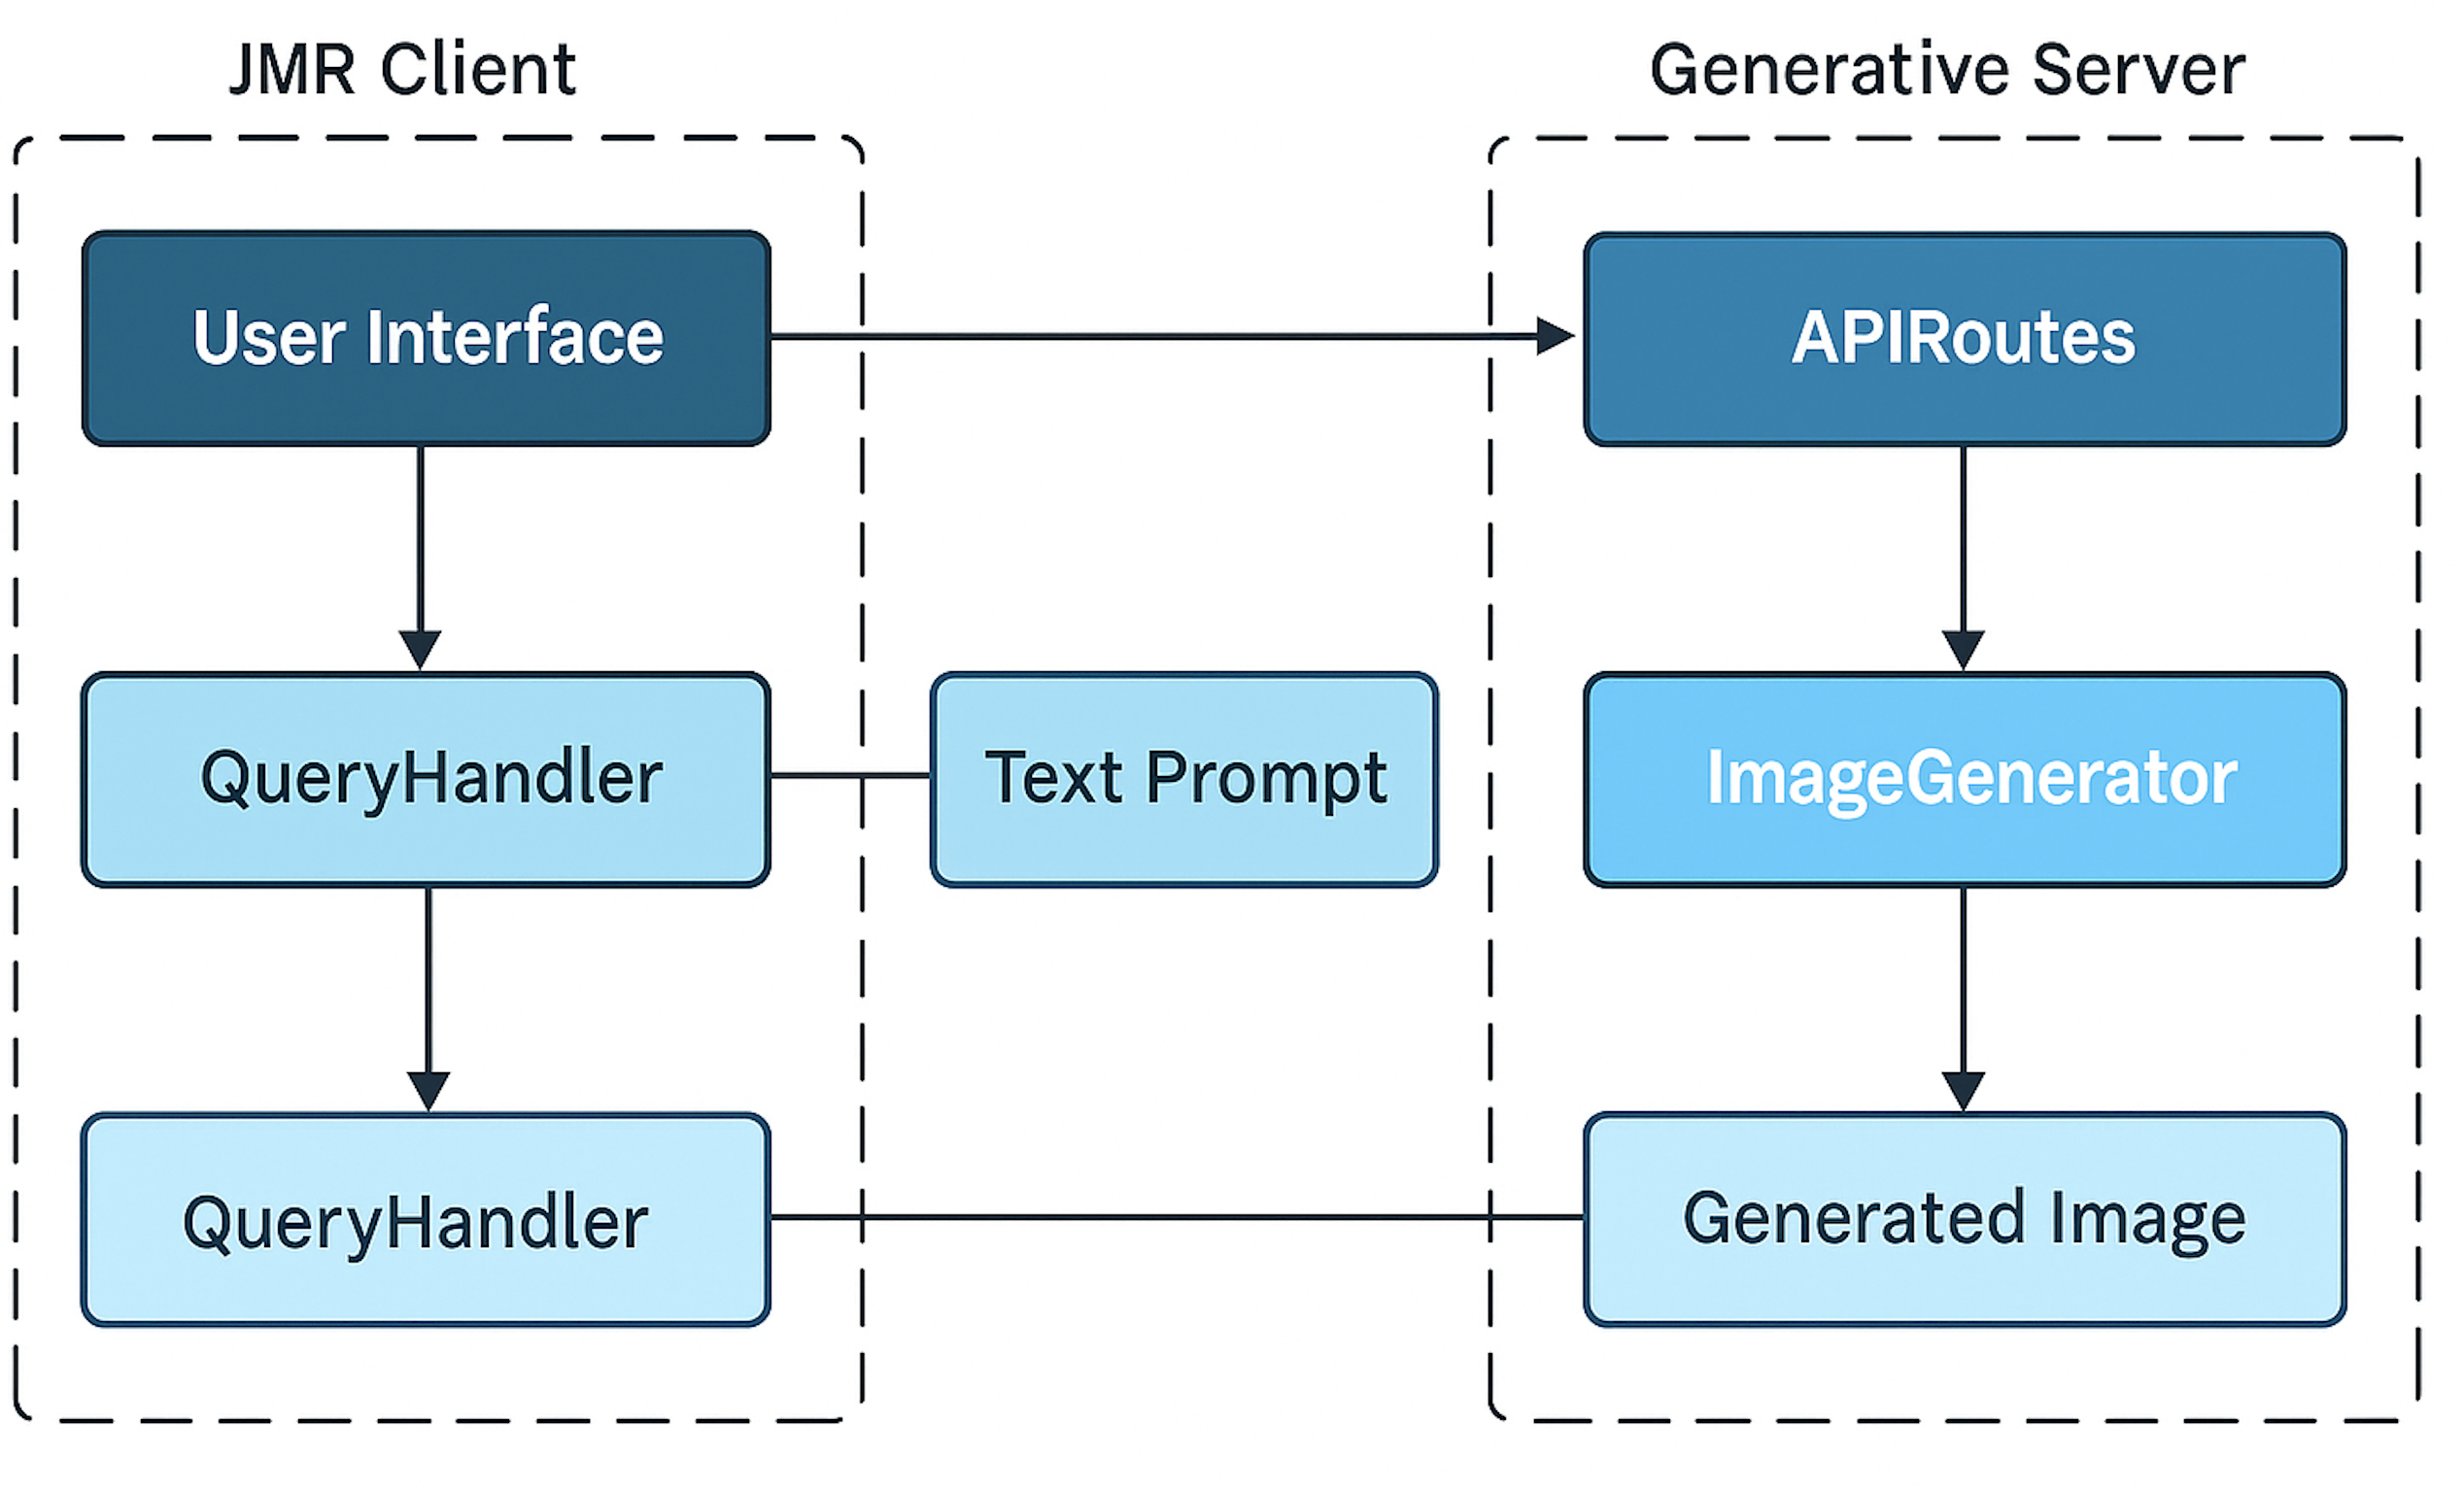
\includegraphics[width=0.7\textwidth]{nueva_arquitectura}
    \caption{Arquitectura lógica del sistema integrado}
    \label{fig:arquitectura-final}
\end{figure}

Esta arquitectura distribuida permite mejorar la mantenibilidad, facilitar la evolución del modelo generativo y adaptar el sistema a diferentes entornos sin afectar a la aplicación principal.

\subsection{Modelo conceptual}

El modelo conceptual del sistema refleja los elementos fundamentales que intervienen en el proceso de generación y búsqueda visual. La Figura~\ref{fig:modelo-conceptual} resume gráficamente este flujo, destacando la interacción entre el usuario, la API generativa y el motor de recuperación visual (CBIR).

\begin{itemize}
    \item \textbf{Usuario:} introduce una descripción textual a través de la interfaz JMR.
    \item \textbf{Prompt o descripción textual:} entrada en lenguaje natural que sirve como semilla para la generación de una imagen.
    \item \textbf{Imagen generada:} salida del modelo de IA a partir del prompt introducido por el usuario.
    \item \textbf{Resultado de búsqueda:} conjunto de imágenes similares recuperadas por el motor CBIR.
    \item \textbf{Configuración del modelo:} conjunto de parámetros que determinan el comportamiento del generador (modelo base, pasos, guidance, etc.).
\end{itemize}

\begin{figure}[H]
    \centering
    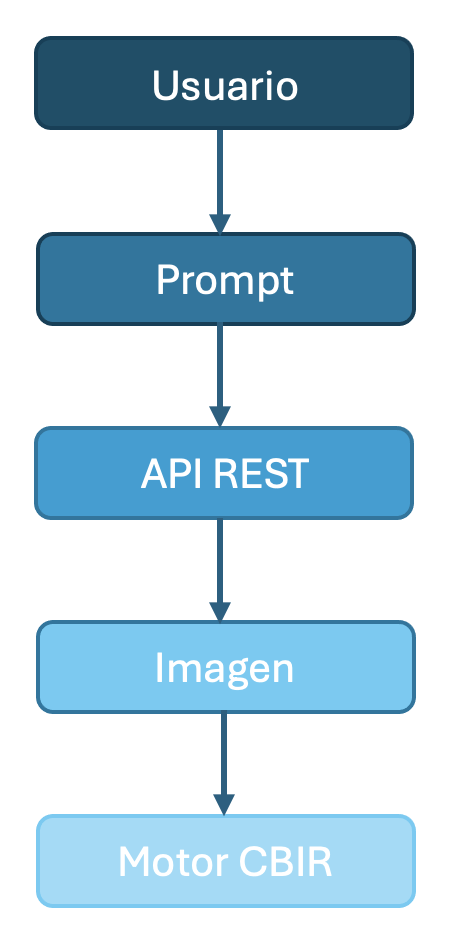
\includegraphics[width=0.2\textwidth]{diagramas/modelo_conceptual.png}
    \caption{Representación esquemática del modelo conceptual del sistema}
    \label{fig:modelo-conceptual}
\end{figure}


Este modelo permitió definir los flujos de información, el diseño de las peticiones API y las entidades clave del sistema.


\subsection{Diseño del modelo de clases}

Dado que el sistema combina componentes en dos lenguajes distintos, se ha documentado por separado el modelo de clases tanto del cliente Java como del servidor Python.

\subsubsection{Modelo de clases en Java}

El modelo de clases Java describe la estructura de la aplicación cliente (JMR) y su interacción con la API de generación de imágenes. En el centro se encuentra la clase \texttt{MainWindow}, que representa la interfaz principal y gestiona el estado de la aplicación, las ventanas internas y la interacción del usuario con los prompts generativos.

La clase \texttt{MainWindow} se conecta con:
\begin{itemize}
\item \texttt{PromptGeneratedImageDescriptor} y \texttt{PromptGeneratedImageDescriptorLocal}, que encapsulan la lógica para realizar consultas generativas, ya sea mediante una API online o una versión local del modelo.
\item \texttt{ImagePromptItem}, que almacena información sobre cada prompt generado y facilita su reutilización.
\end{itemize}

Estas clases se encargan de gestionar tanto los datos visuales como los metadatos asociados (prompts, rutas, respuestas HTTP). Además, se incluyen clases auxiliares como \texttt{Circulo}, utilizadas en otras funcionalidades del sistema visual de JMR, pero que se mantienen desacopladas del módulo generativo.

Este diseño modular permite que la interfaz pueda comunicarse con diferentes fuentes de generación de imágenes sin modificar la lógica principal, facilitando la escalabilidad y la extensión futura del sistema.

\begin{figure}[H]
\centering
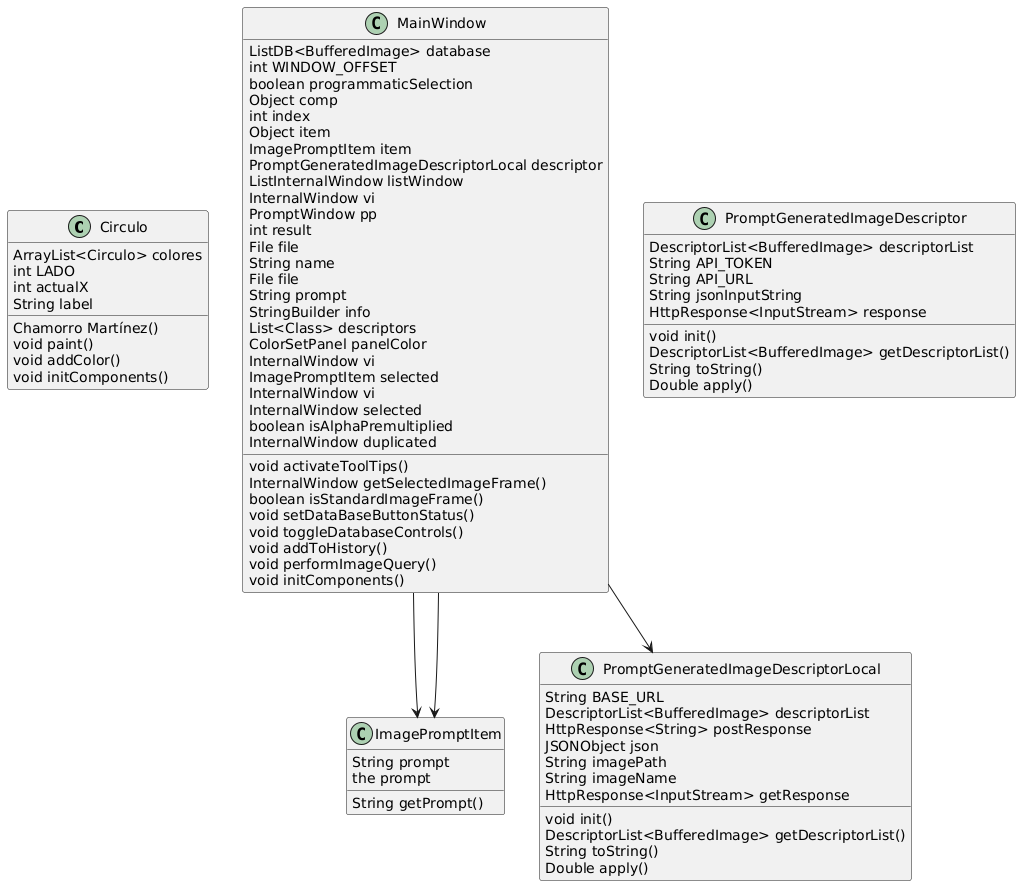
\includegraphics[width=0.9\textwidth]{diagrama_clases_java}
\caption{Diagrama de clases del módulo de integración en Java}
\label{fig:clases-java}
\end{figure}

\subsubsection{Modelo de clases en Python}

El modelo de clases en Python, representado como una abstracción de los módulos funcionales, refleja la lógica interna del sistema generativo. En el centro se encuentra la clase conceptual \texttt{DogTrainer}, que agrupa todos los elementos necesarios para el entrenamiento y generación de imágenes mediante DreamBooth.

Esta clase maneja:
\begin{itemize}
\item La descarga y filtrado del dataset (\texttt{download\_and\_extract\_dataset()}, \texttt{select\_images()}).
\item El entrenamiento del modelo personalizado (\texttt{train\_dreambooth()}).
\item La generación de imágenes y compresión de resultados (\texttt{generate\_images()}, \texttt{zip\_results()}).
\end{itemize}

Además, se incluye la clase \texttt{DogDataset}, que estructura el conjunto de datos utilizado para el entrenamiento, y \texttt{GenerateRequest}, que define los parámetros necesarios para realizar una petición de generación.

En cuanto a la API, se representan los distintos módulos como clases con sus funciones principales:
\begin{itemize}
\item \texttt{ModelOperations} para gestión de modelos (upload, delete, list),
\item \texttt{ImageOperations} para generación y descarga de imágenes,
\item \texttt{Validation} para la comprobación estructural de los modelos subidos.
\end{itemize}

Este enfoque facilita la mantenibilidad del sistema y su extensión a nuevas funcionalidades, garantizando una separación clara entre el entrenamiento, la generación y la exposición mediante API.

\begin{figure}[H]
\centering
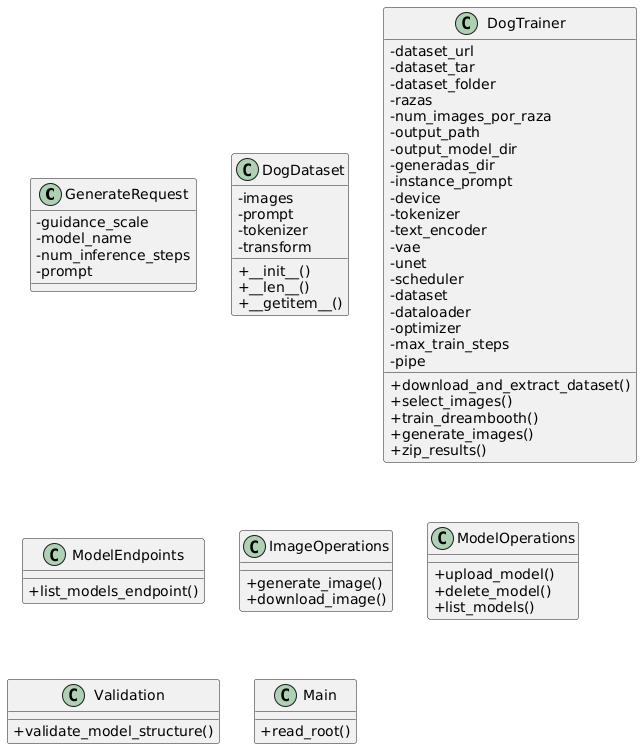
\includegraphics[width=0.75\textwidth]{diagrama_clases_python}
\caption{Diagrama de clases del sistema generativo en Python}
\label{fig:clases-python}
\end{figure}


\subsection{Diseño de la interfaz}
El diseño de la interfaz de usuario ha sido un componente clave para facilitar la interacción con el sistema de generación y búsqueda de imágenes. Este apartado presenta la evolución del diseño, desde los primeros esquemas conceptuales hasta el prototipo final interactivo. Se parte del análisis de flujo de interacción, se muestran los bocetos iniciales y wireframes funcionales, y finalmente se presenta el prototipo desarrollado en Figma. Además, se analizan los principios de usabilidad aplicados para garantizar una experiencia fluida e intuitiva para el usuario final.

\subsubsection{Diagrama de flujo de interacción}
El siguiente diagrama de flujo describe la secuencia de operaciones que se ejecutan desde la introducción del prompt por parte del usuario hasta la obtención de los resultados visuales. Este flujo ilustra la lógica general del sistema, destacando las decisiones clave y la coordinación entre los distintos módulos (interfaz gráfica, API de generación y sistema CBIR).

\begin{figure}[H]
    \centering
    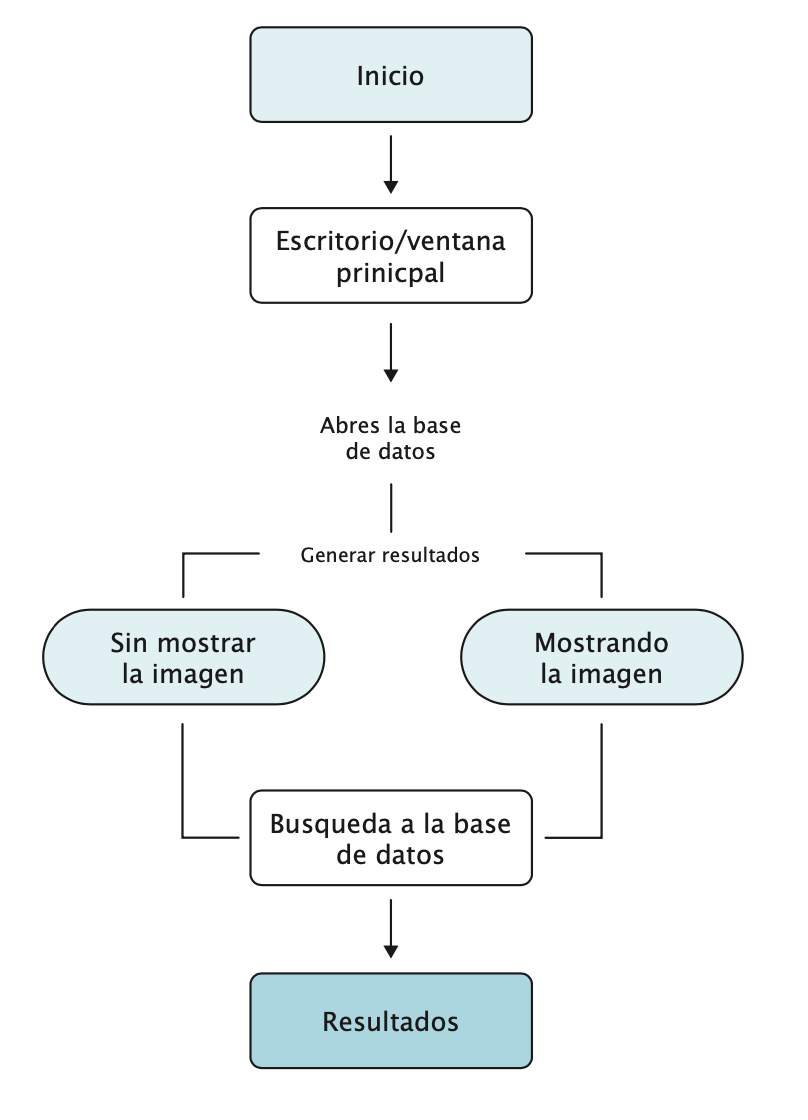
\includegraphics[width=0.6\textwidth]{diagramas/diagrama_flujo.png}
    \caption{Flujo de interacción entre el usuario, la API generativa y el sistema CBIR}
    \label{fig:flujo-interaccion}
\end{figure}

\subsubsection{Bocetos}

Los primeros bocetos se realizaron a mano con el objetivo de definir la estructura inicial de la interfaz, priorizando la disposición de los componentes principales: el área de entrada del prompt, el botón de generación, la galería de resultados y las opciones adicionales de filtrado o guardado. Estos bocetos permitieron una exploración rápida de ideas antes de pasar a herramientas digitales.

El primer boceto muestra la vista general del escritorio o ventana principal de la aplicación. En la parte superior se encuentra una barra de herramientas con botones y opciones de interacción. La zona central queda libre para cargar ventanas internas según las acciones del usuario, como la generación o visualización de imágenes.

\begin{figure}[H]
    \centering
    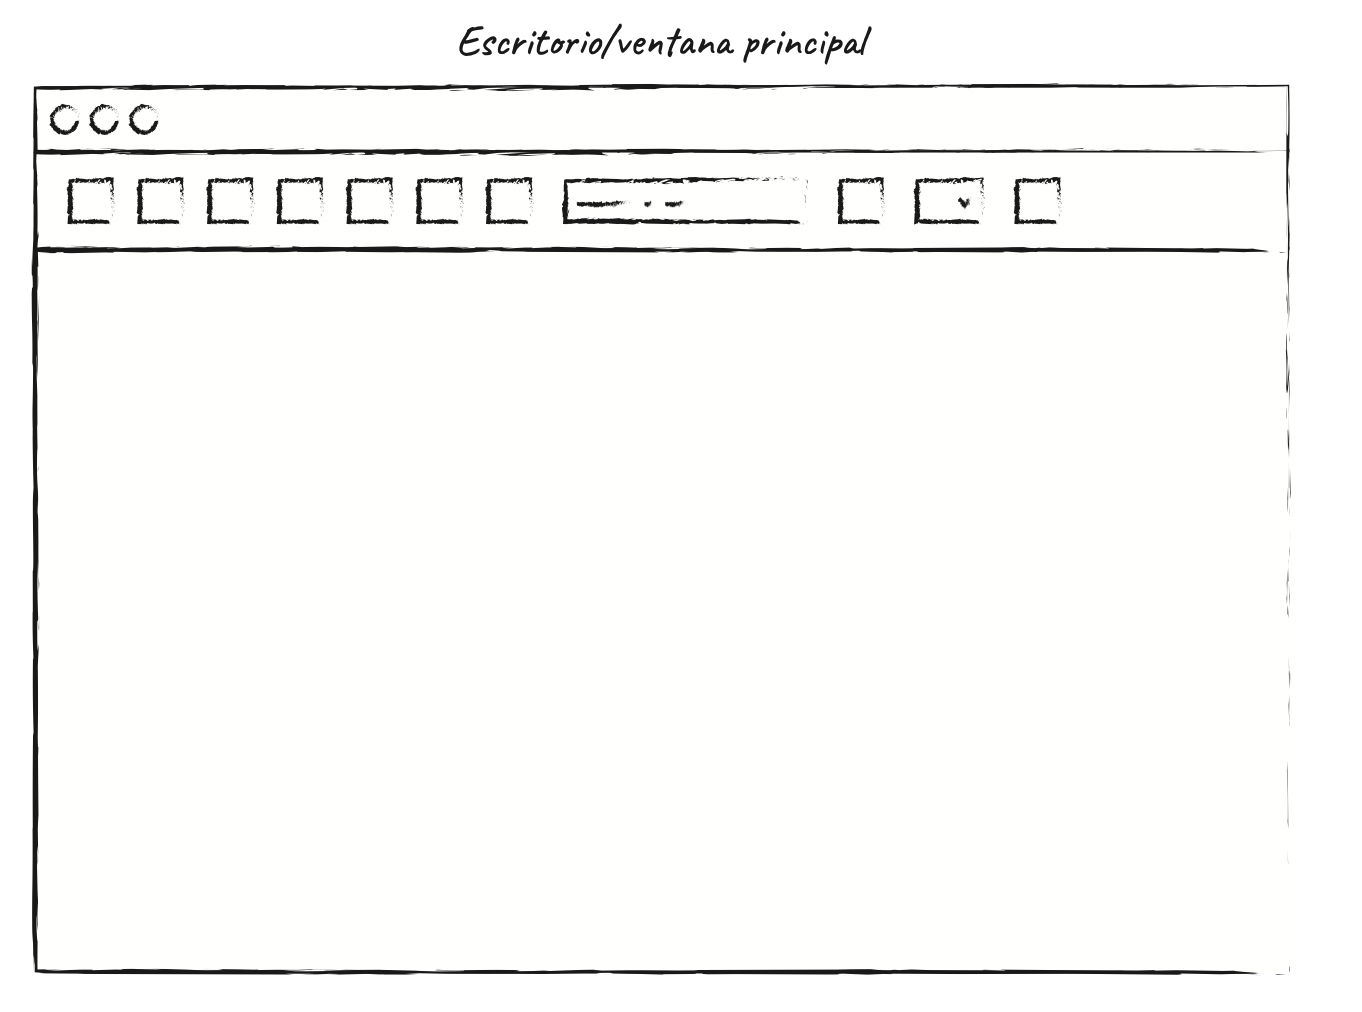
\includegraphics[width=0.7\textwidth]{bocetos/boceto1.png}
    \caption{Boceto: propuesta inicial del layout general}
    \label{fig:boceto1}
\end{figure}

El segundo boceto representa la ventana de generación de imagen. Esta aparece superpuesta sobre el escritorio y contiene una zona de entrada de texto donde el usuario puede escribir el prompt, junto con un botón de acción y una barra de carga que indica el estado del proceso de generación.

\begin{figure}[H]
    \centering
    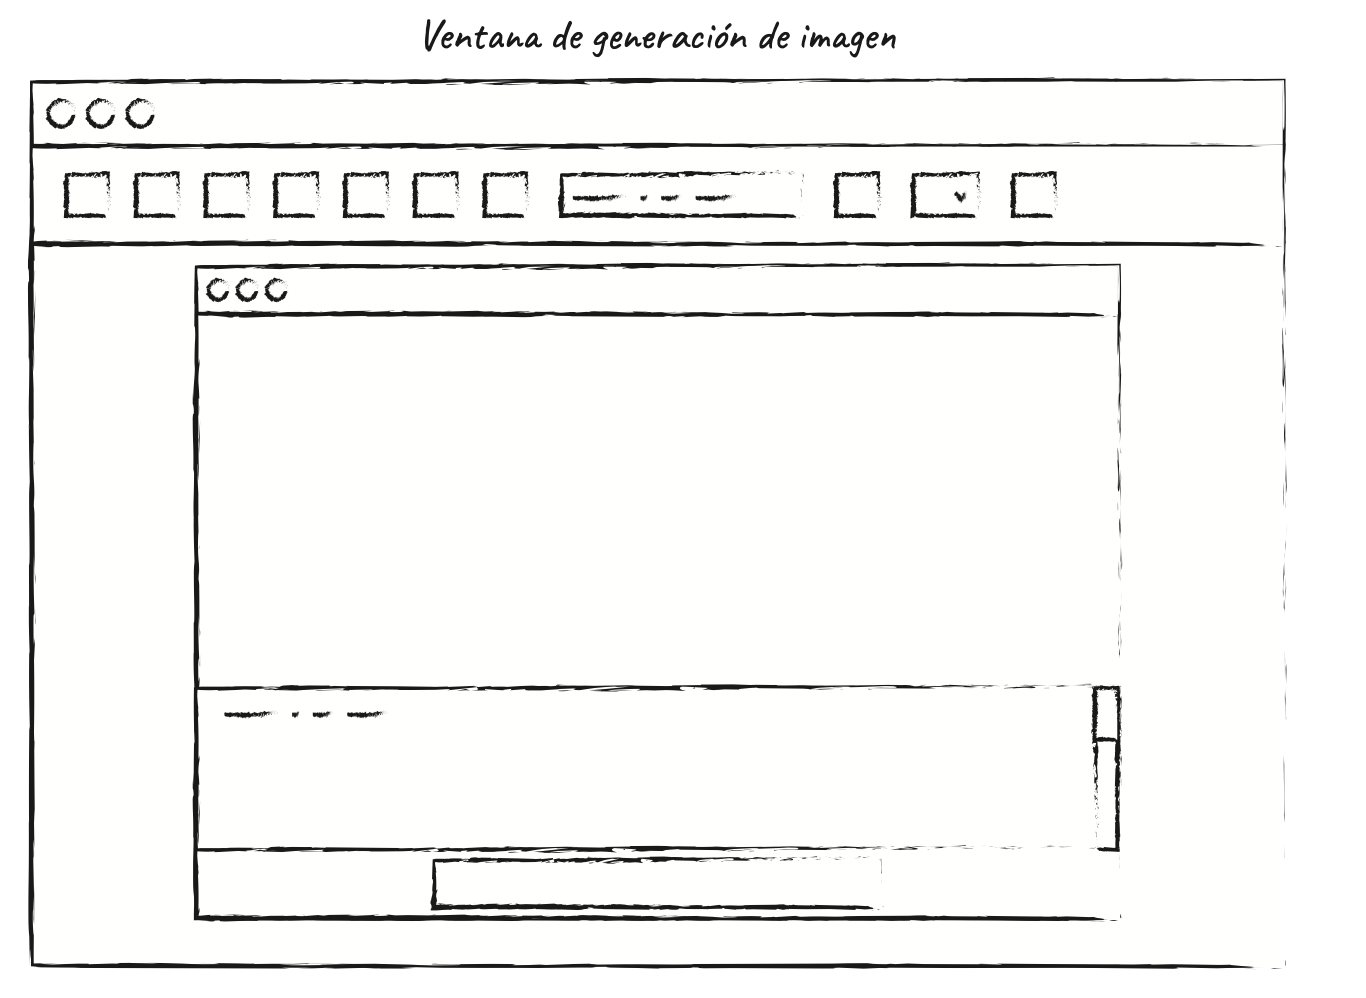
\includegraphics[width=0.7\textwidth]{bocetos/boceto2.png}
    \caption{Boceto: navegación entre secciones}
    \label{fig:boceto2}
\end{figure}

El tercer boceto corresponde a la vista de resultados generados. En la parte superior se visualiza una galería de imágenes miniatura, mientras que en la zona inferior se muestra una imagen ampliada seleccionada por el usuario. Este diseño facilita la exploración visual y la interacción posterior, como aplicar descriptores o realizar búsquedas visuales.

\begin{figure}[H]
    \centering
    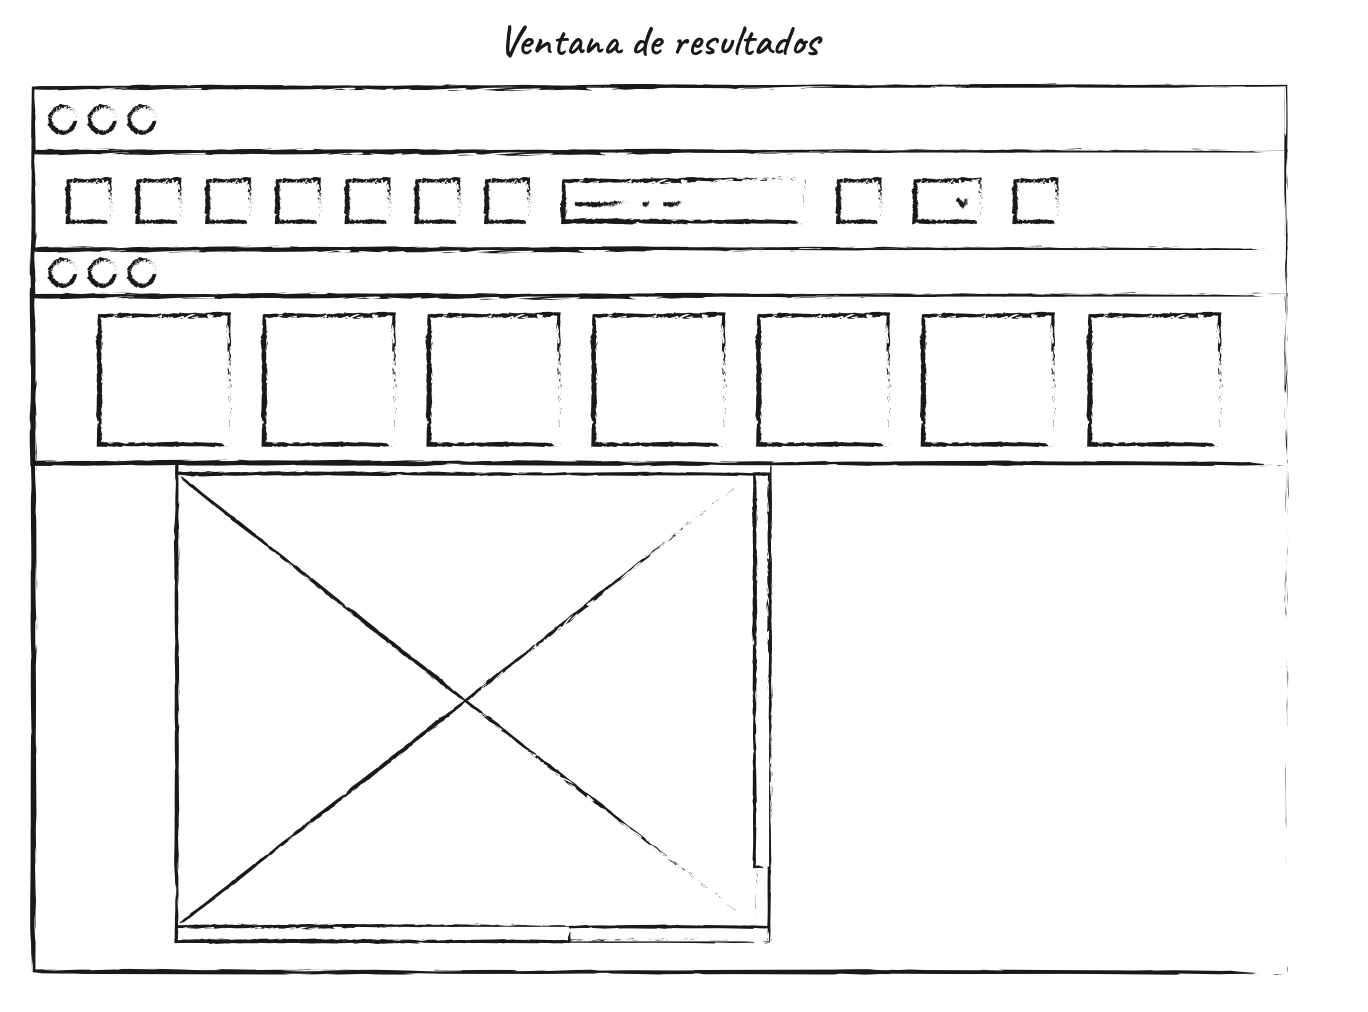
\includegraphics[width=0.7\textwidth]{bocetos/boceto3.png}
    \caption{Boceto: detalle de interacción en la vista de resultados}
    \label{fig:boceto3}
\end{figure}


\subsubsection{Wireframes}

A partir de los bocetos iniciales, se desarrollaron wireframes de baja fidelidad utilizando herramientas digitales. Estos permitieron refinar la experiencia de usuario, definir la jerarquía visual de cada componente y estructurar la navegación entre secciones clave del sistema.

La primera pantalla corresponde al escritorio o ventana principal del sistema. En ella se muestra la interfaz base del entorno JMR, con su barra de herramientas y el área central donde se mostrarán las distintas ventanas internas.

\begin{figure}[H]
    \centering
    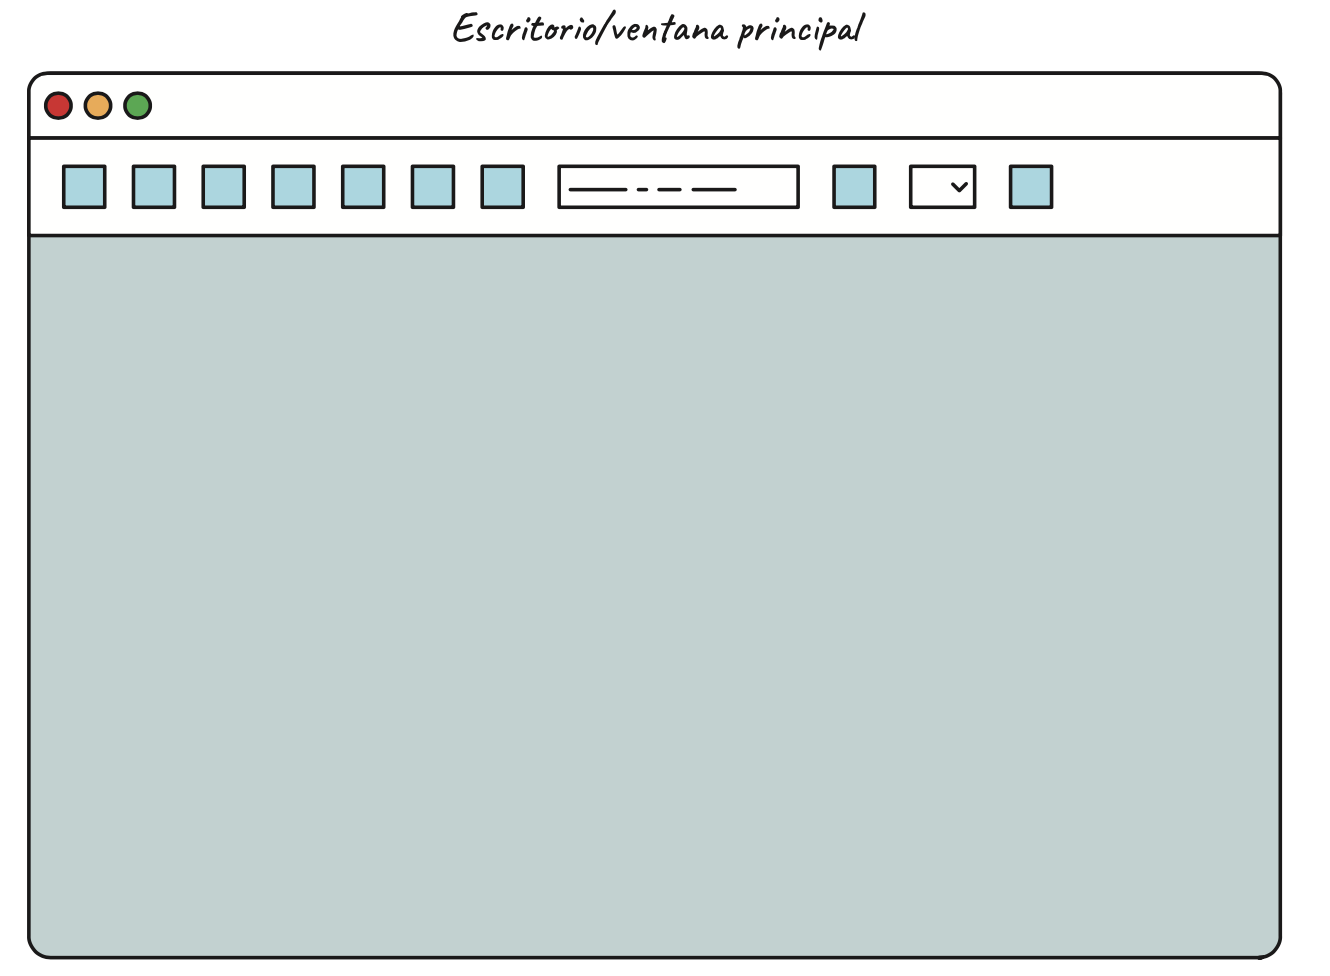
\includegraphics[width=0.65\textwidth]{wireframes/wireframe1.png}
    \caption{Wireframe: pantalla principal con área de generación}
    \label{fig:wireframe1}
\end{figure}

La segunda imagen representa la ventana de generación de imagen. Esta ventana se abre dentro del escritorio cuando el usuario decide introducir un prompt. Incluye un área de visualización de la imagen generada, un campo de entrada de texto y un botón de acción.

\begin{figure}[H]
    \centering
    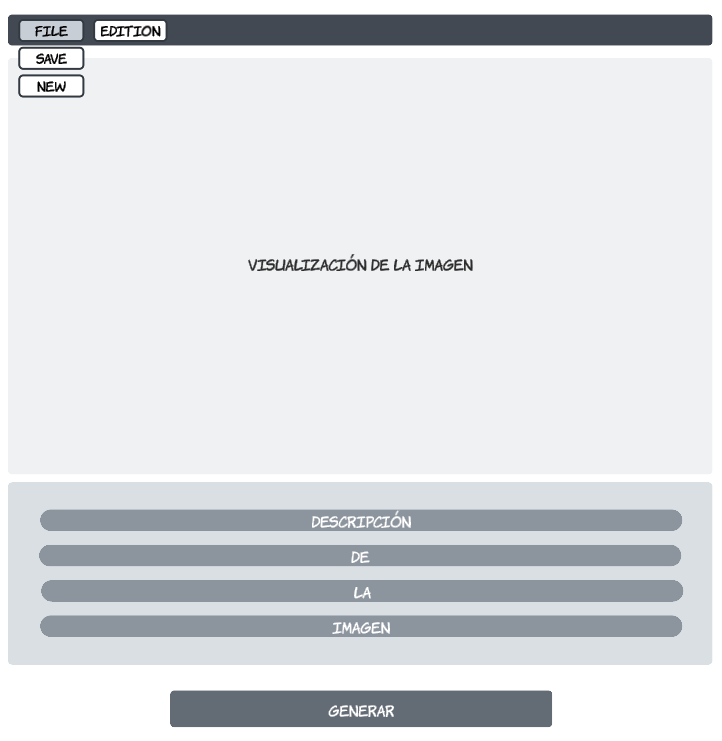
\includegraphics[width=0.65\textwidth]{wireframes/wireframe2.png}
    \caption{Wireframe: visualización detallada de una imagen generada}
    \label{fig:wireframe3}
\end{figure}

El tercer wireframe muestra la pantalla de resultados, donde se visualiza la imagen generada y las imágenes recuperadas mediante el sistema CBIR. En la parte superior se encuentra la galería de resultados similares y, debajo, una vista ampliada de la imagen seleccionada.

\begin{figure}[H]
    \centering
    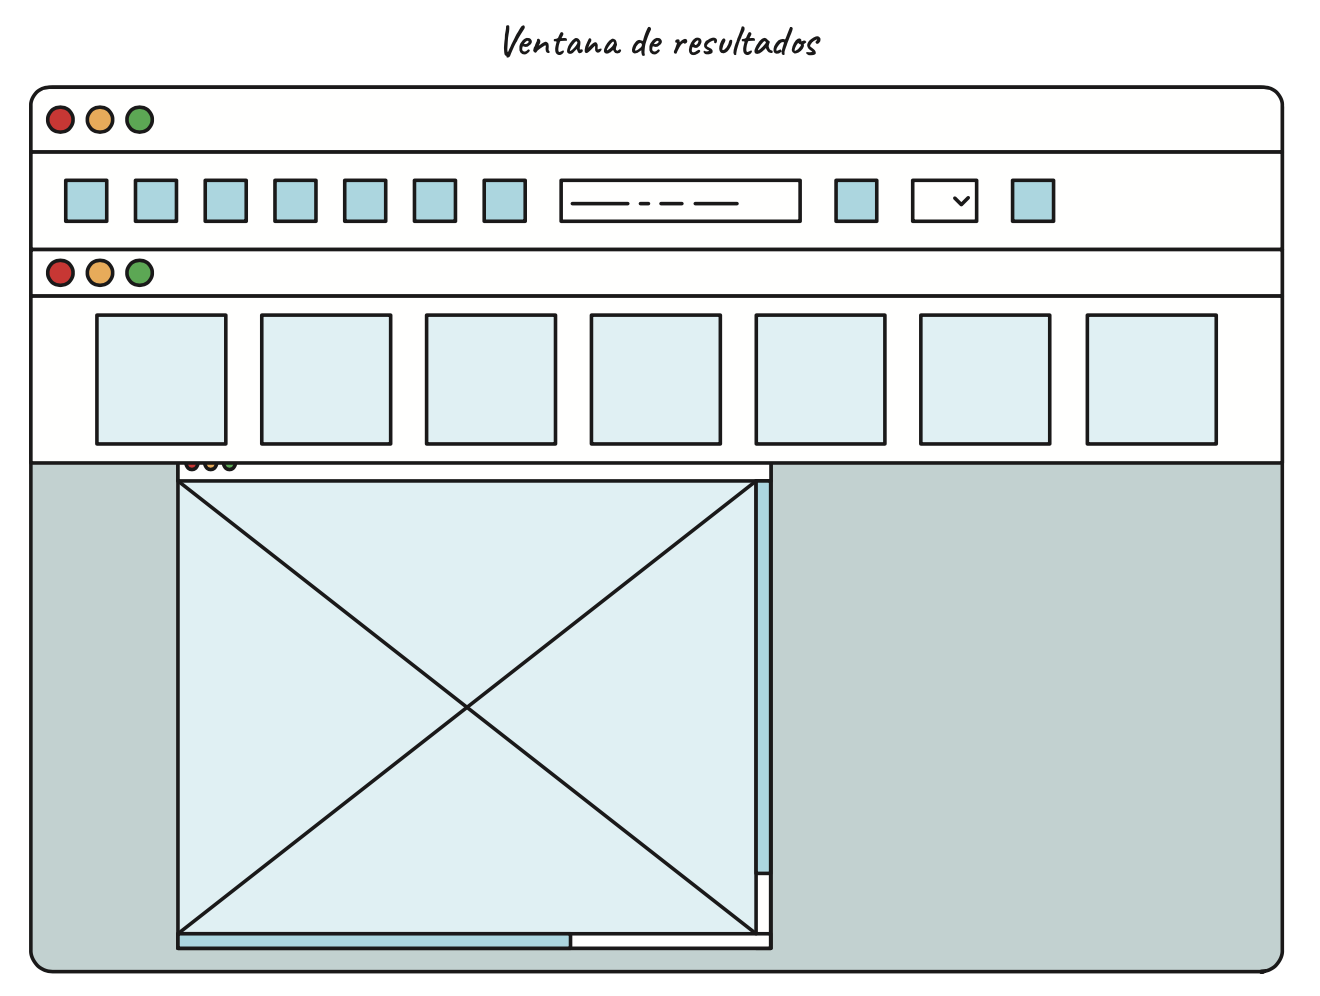
\includegraphics[width=0.65\textwidth]{wireframes/wireframe3.png}
    \caption{Wireframe: pantalla de resultados con opciones de filtrado}
    \label{fig:wireframe2}
\end{figure}

\subsubsection{Prototipo en Figma}

Como parte final del diseño de la interfaz, se construyó un prototipo funcional en Figma basado en los wireframes anteriores. Este prototipo permitió simular la navegación entre ventanas y validar la experiencia de usuario en un entorno gráfico realista.

La interacción está compuesta por distintas pantallas: la ventana principal de escritorio, la ventana emergente de generación, la vista con imagen generada, la galería de resultados y el histórico de prompts. También se definieron transiciones claras entre cada pantalla, incluyendo retroalimentación tras la generación o selección de imágenes. 

Este flujo fue clave para observar posibles puntos de mejora en usabilidad y validar la navegación global del sistema antes de implementarlo.

\begin{figure}[H]
    \centering
    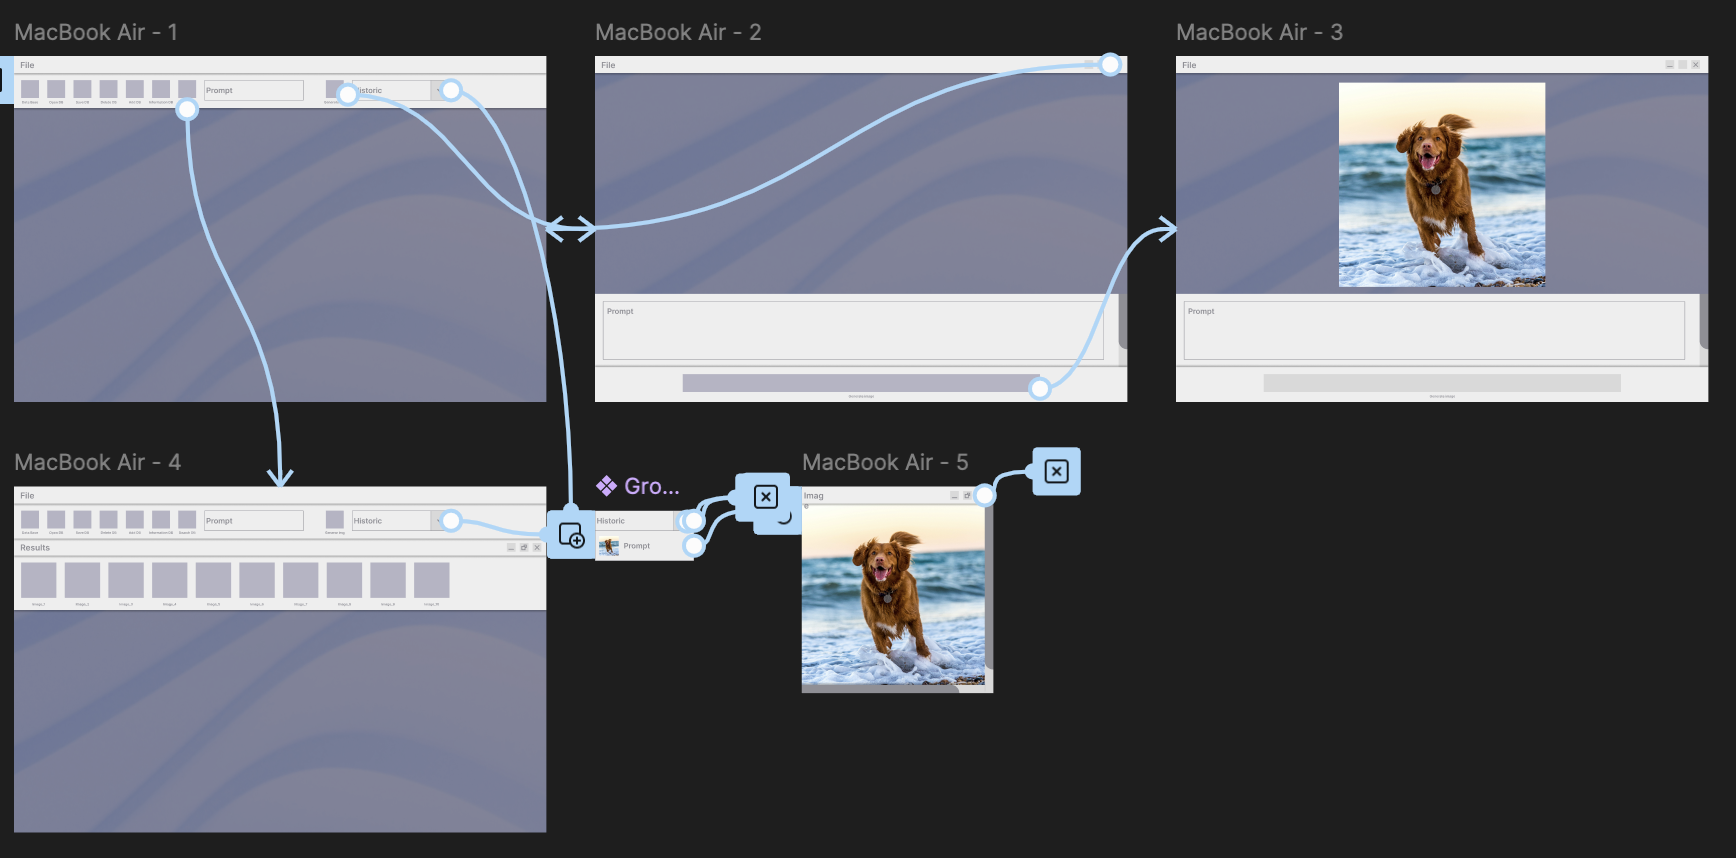
\includegraphics[width=1\textwidth]{figma/general.png}
    \caption{Vista general del flujo de navegación entre pantallas del prototipo en Figma}
    \label{fig:figma-prototype}
\end{figure}

Las capturas detalladas de las pantallas y sus interacciones están disponibles en el Anexo~\ref{anexo:figma}.

\subsubsection{Usabilidad}

El diseño de la interfaz se ha guiado por principios fundamentales de usabilidad con el objetivo de ofrecer una experiencia accesible, eficiente y satisfactoria para todo tipo de usuarios, independientemente de su nivel técnico. A partir de las historias de usuario definidas (HU1 y HU2), se identificaron tres necesidades clave: introducir descripciones textuales de forma clara, visualizar resultados generados de forma comprensible, y reutilizar esas imágenes para buscar contenido visual similar en la base de datos.

Con base en estos objetivos, se aplicaron los siguientes principios de diseño centrado en el usuario:

\begin{itemize}
    \item \textbf{Interacción simple y directa:} La interfaz principal presenta solo los elementos esenciales para la tarea principal: un campo para introducir el prompt, un botón para iniciar la generación y un área de visualización de la imagen resultante. Esta simplicidad evita la sobrecarga cognitiva y facilita que el usuario comprenda rápidamente cómo usar el sistema sin necesidad de asistencia externa.

    \item \textbf{Retroalimentación inmediata y comprensible:} Tras introducir el prompt, el sistema proporciona indicadores visuales (como animaciones de carga) que confirman que la solicitud está siendo procesada. Al completarse la generación, la imagen se muestra de forma destacada, acompañada de una acción clara para continuar con el flujo (por ejemplo, usarla como consulta en el sistema CBIR). Esto mantiene al usuario informado en todo momento y refuerza su confianza en el sistema.

    \item \textbf{Consistencia visual y funcional:} Se respetaron convenciones de diseño ampliamente reconocidas: uso de etiquetas descriptivas, alineaciones verticales, botones claramente diferenciados y jerarquía visual basada en el tamaño y el color. Esto reduce el tiempo de aprendizaje y evita comportamientos inesperados.

    \item \textbf{Accesibilidad y legibilidad:} Se priorizó el uso de tipografía clara, buen contraste entre texto y fondo, y tamaños adecuados de los elementos interactivos para facilitar el uso tanto en pantallas grandes como en dispositivos de menor tamaño. Asimismo, se evitó el uso de términos técnicos complejos, apostando por un lenguaje neutro y comprensible.

    \item \textbf{Minimización de errores y puntos de fricción:} El flujo está diseñado para prevenir errores comunes, como el envío de prompts vacíos o duplicados. Además, en caso de fallo (por ejemplo, si no se genera una imagen), el sistema informa con mensajes explicativos que permiten al usuario comprender lo ocurrido y actuar en consecuencia.
\end{itemize}

En conjunto, estas decisiones de diseño han permitido construir una interfaz que no solo es funcional, sino también intuitiva y centrada en las necesidades reales del usuario. Esto resulta especialmente importante en un sistema como este, donde se combinan tecnologías avanzadas (IA generativa y recuperación de imágenes) con una interacción aparentemente simple basada en lenguaje natural.
